%\newpage

\section{Problem Definition}
\label{sec:problem-definition}
%\guy{Can someone check Sections 3-4-5? Especially the formulations}

Our network system (NS) syntax is defined as follows: 
%of Fig.~\ref{fig:syntax}.

\[
\begin{aligned}
	\mathbf{Expression}\quad e ::={}&{} \\
	&0 \mid 1 \mid 2 \mid \dots 
	&&\grammartag{Numeric constants}\\
	&\nondet
	&&\grammartag{Nondeterministic value: 0 or 1}\\
	&x := e
	&&\grammartag{Write to local variable}\\
	&x
	&&\grammartag{Read from local variable}\\
	&X := e
	&&\grammartag{Write to global variable}\\
	&X
	&&\grammartag{Read from global variable}\\
	&e_1 == e_2
	&&\grammartag{Equality test}\\
	&e_1 ; e_2
	&&\grammartag{Sequencing}\\
	&\ifkw(e_1)\{e_2\}\elsekw\{e_3\}
	&&\grammartag{Conditional}\\
	&\whilekw(e_1)\{e_2\}
	&&\grammartag{While loop}\\
	&\yieldkw
	&&\grammartag{Yields to scheduler}\\[1em]
	\mathbf{Program}\quad p ::={}&{} \\
	&\requestkw\ name_1\{e_1\}
	&&\grammartag{Set of request handlers}\\
	&\quad\vdots\\
	&\requestkw\ name_n\{e_n\}
\end{aligned}
\]

%
%
%\begin{figure}[!htbp]
%    \begin{align*}
%    \mathbf{Expression}\quad e ::= &&& \\
%       | & \quad 0 \mid 1 \mid 2 \mid \ldots                                && \grammartag{Numeric constants} \\
%       | & \quad \nondet                                 && \grammartag{Nondeterministic value: 0 or 1}\\
%       | & \quad x := e                            && \grammartag{Write to local variable field} \\
%       | & \quad x                                 && \grammartag{Read from local variable field} \\
%       | & \quad X := e                            && \grammartag{Write to global  variable} \\
%       | & \quad X                                 && \grammartag{Read from global  variable} \\
%       | & \quad e_1 == e_2                        && \grammartag{Equality test} \\
%       | & \quad e_1 ; e_2                         && \grammartag{Sequencing} \\
%       | & \quad \ifkw(e_1)\{\ e_2\ \}\elsekw\{\ e_3\ \} && \grammartag{Conditional} \\
%       | & \quad \whilekw(e_1)\{\ e_2\ \}              && \grammartag{While loop} \\
%       | & \quad \yieldkw                      && \grammartag{Yields to scheduler}\\[1em]
%    \mathbf{Program}\quad p ::=
%        & \quad \requestkw\ name_1\ \{\ e_1\ \}&&\grammartag{Set of request handlers}\\[-0.5em]
%        & \quad \qquad \vdots &&\\
%        & \quad \requestkw\ name_n\ \{\ e_n\ \}\ 
%    \end{align*}
%    \caption{Syntax of expressians and programs}
%    \label{fig:syntax}
%\end{figure}
    %
This NS setting is motivated by software-defined networking systems. Specifically, spawning a request corresponds to sending a packet, with each local variable mapped to a unique packet header field; global variables correspond to variables on programmable switches, as they are shared among all packets (threads) of the system, visiting the switch. Throughout this section, we will refer to packets/threads/requests interchangeably. 
    
   
A Network System $\mathcal{N}$ is a tuple $(G, L, \mathit{REQ}, \mathit{RESP}, g_0, \delta, \mathit{req}, \mathit{resp})$ where:
\begin{itemize}
\item $G$ is a set of global states (each is one possible assignment of global variables simultaneously) 
\item $L$ is a set of local states representing request/thread contents (local variable values and ``remaining program'' to execute)
\item $\mathit{REQ}$ is a set of request events (each marked {\color{ForestGreen}$\blacklozenge_\text{req}$})
\item $\mathit{RESP}$ is a set of response events (each marked {\color{red}$\blacklozenge_\text{resp}$})
\item $g_0 \in G$ is the initial global state
\item $\mathit{req} \subseteq \mathit{REQ} \times L$ is a request transition relation, which describes which request spawns which thread (packet)
\item $\mathit{resp} \subseteq L \times \mathit{RESP}$ is a response transition relation, which describes which thread turns into which responses
\item $\delta \subseteq (G \times L) \times (G \times L)$ is a transition relation for thread processing, which describes an atomic step of processing that may change the (shared) global state and the (private) thread-local state.
\end{itemize}




\begin{figure}[t]
    \centering
    \renewcommand{\arraystretch}{1.6}
    \[
    \begin{array}{c}
    \textbf{States and Transitions:}
    \\
    \quad
    \text{A (global) \emph{network state} is a triple }(g,\mathcal{P},M)\text{ where:}
    \\
    \quad
    g \in G \text{ is the current global state,}
    \\
    \quad
    \mathcal{P} \in \text{Multiset}(L \times \mathit{REQ}) \text{ is a multiset of in-flight requests (threads),}
    \\
    \quad
    M \in \text{Multiset}(\mathit{REQ} \times \mathit{RESP}) \text{ is a multiset of request/response pairs already completed.}
    \end{array}
    \]

    \[
    \begin{array}{c}
    \textbf{Initial state:}
    \\
    \quad (g_0,\,\varnothing,\,\varnothing)
    \end{array}
    \]

    \[
    \begin{array}{c}
    \textbf{Transition rules:}
    \\[1em]
    \text{(New Request)}\quad\infer{
    ({\color{ForestGreen}\blacklozenge_\text{r}},\ell)\,\in\,\mathit{req}
    }
    {(g,\;\mathcal{P},\;M) \;\longrightarrow\; (g,\;\mathcal{P} \uplus \{(\ell,{\color{ForestGreen}\blacklozenge_\text{r}})\},\;M)}
    \\[2em]
    \text{(Processing Step)}\quad\infer{
    ((g,\ell),\,(g',\ell')) \,\in\, \delta
    }
    {(g,\;\mathcal{P} \uplus \{(\ell,{\color{ForestGreen}\blacklozenge_\text{r}})\},\;M) \;\longrightarrow\; (g',\;\mathcal{P} \uplus \{(\ell',{\color{ForestGreen}\blacklozenge_\text{r}})\},\;M)}
    \\[2em]
    \text{(Response)}\quad\infer{
    (\ell,{\color{red}\blacklozenge_\text{s}})\,\in\,\mathit{resp}
    }
    {(g,\;\mathcal{P} \uplus \{(\ell,{\color{ForestGreen}\blacklozenge_\text{r}})\},\;M) \;\longrightarrow\; (g,\;\mathcal{P},\;M \uplus \{({\color{ForestGreen}\blacklozenge_\text{r}},{\color{red}\blacklozenge_\text{s}})\})}
    \end{array}
    \]

    \[
    \begin{array}{c}
    \textbf{Complete runs:}
    \\
    \quad (g_0,\,\varnothing,\,\varnothing) \;\longrightarrow\; (g_1,\,\mathcal{P}_1,\,M_1) \;\longrightarrow\; \cdots \;\longrightarrow\; (g_n,\,\mathcal{P}_{n-1},\,M_{n-1}) \;\longrightarrow\; (g_n,\,\varnothing,\,M_n)
    \\[1em]
    \textbf{Interleaved run: } \text{the } \mathcal{P}_i \text{ can have more than one request, and } \mathcal{P}_n = \varnothing \\
    \textbf{Serial run: } \text{ each } \mathcal{P}_i \text{ has at most one request, and } \mathcal{P}_n = \varnothing\\
    \text{Int}(\mathcal{N}) = \{ M \in \text{Multiset}(\mathit{REQ} \times \mathit{RESP}) \mid \exists \text{ interleaved run } (g_0,\,\varnothing,\,\varnothing) \;\longrightarrow^*\; (g_n,\,\varnothing,\,M) \}\\
    \text{Ser}(\mathcal{N}) = \{ M \in \text{Multiset}(\mathit{REQ} \times \mathit{RESP}) \mid \exists \text{ serial run } (g_0,\,\varnothing,\,\varnothing) \;\longrightarrow^*\; (g_n,\,\varnothing,\,M) \}\\
    \end{array}
    \]

    \caption{State-transition rules for executions of
    \(\mathcal{N} = (G, L, \mathit{REQ}, \mathit{RESP}, g_0, \delta, \mathit{req}, \mathit{resp})\).
    A transition \(\longrightarrow\) modifies the triple \((g,\mathcal{P}, M)\) by either (1) introducing a new request, (2) processing a request step via \(\delta\), or (3) consuming a request to produce its response.  When no more steps are possible, the result set \(M\) is the final multiset of request/response pairs that arose during the run.
    Runs are called \emph{serial} if there is at most one packet in flight at any time, whereas \emph{interleaved} runs may have multiple packets in flight at once.}
    \label{fig:network-transitions}
\end{figure}

%\guy{Nicolas/Jules can you take a look at the other definition that I masked in the latex below? Is the current one good enough?}

%\begin{definition}[Interleaved executions \(\mathrm{Int}(\mathcal{N})\)]
%    Let \(\mathcal{N} = (G, L, \mathit{Req}, \mathit{Res}, g_0, \delta, \mathit{req}, \mathit{resp})\).
%    An \emph{interleaved execution} begins in global state \(g = g_0\) with no packets in flight.
%    At any point, one may:
%    \begin{itemize}
%        \item introduce a new request \(r \in \mathit{Req}\), producing an in-flight packet \(\ell \in L\) if \((r,\ell) \in \mathit{req}\);
%        \item take an in-flight packet \(\ell\) and transition \(\ell \mapsto \ell'\) and \(g \mapsto g'\) if \(((g,\ell),(g',\ell'))\in\delta\);
%        \item consume an in-flight packet \(\ell\) to produce a response \(s\) if \((\ell,s)\in \mathit{resp}\).
%    \end{itemize}
%    Each request \(r\) must eventually yield exactly one corresponding response \(s\) in a valid execution.
%    The set of all finite multisets of \((r,s)\) pairs realizable by such interleavings is:
%    \[
%        \mathrm{Int}(\mathcal{N})
%        \;=\;
%        \bigl\{
%        M \;\in\; \text{Multiset}(\mathit{Req}\times \mathit{Res})
%        \;\mid\;
%        M \text{ is realized by some interleaved run of }\mathcal{N}
%        \bigr\}.
%    \]
%\end{definition}
%
%\begin{definition}[Serial executions \(\mathrm{Ser}(\mathcal{N})\)]
%In a \emph{serial} execution, requests are processed one at a time:
%\begin{enumerate}
%    \item Start in \(\,g_0\).
%    \item Take a single request \(r\in \mathit{Req}\), convert it to a packet, process that packet until a response \(s\in \mathit{Res}\) is produced.
%    \item Update the global state accordingly and repeat with the next request.
%\end{enumerate}
%No two requests overlap in processing.
%The set of all finite multisets of \((r,s)\) pairs realizable by such one-at-a-time runs is:
%\[
%    \mathrm{Ser}(\mathcal{N})
%    \;=\;
%    \bigl\{
%    M \;\in\; \text{Multiset}(\mathit{Req}\times \mathit{Res})
%    \;\mid\;
%    M \text{ is realized by some serial run of }\mathcal{N}
%    \bigr\}.
%\]
%\end{definition}



%\begin{theorem}[Serial Equivalence]
%\label{thm:ser-eq-ser}
%Whether
%\(
%    \mathrm{Ser}(\mathcal{N}) \;=\; \mathrm{Ser}(\mathcal{N})
%\)
%holds is decidable.
%\end{theorem}
%
%\begin{theorem}[Interleaved Equivalence]
%\label{thm:int-eq-int}
%Whether
%\(
%    \mathrm{Int}(\mathcal{N}) \;=\; \mathrm{Int}(\mathcal{N})
%\)
%holds is undecidable.
%\end{theorem}

\subsection{NS Example: Non-Serializability }
\label{sec:ns-non-serializable}

Recall the code snippet from the simple, non-serializable example presented in Listing~\ref{lst:MotivatingExample2NonSer}. We can represent its NS with the following mapping:

\begin{itemize}
\item 
The set $G$ is defined as $G=\{[X=0], [X=1]\}$

\item 
The initial global $g_0$ state is defined as $g_0 = [X=0]$.

\item 
We define $L$ as all pairs of local states (assignments such as $[y=0], [y=1]$) and ``remaining'' programs.

\item 
The set of requests is $REQ = \{{\color{ForestGreen}\blacklozenge_\text{main}}\}$

\item 
The set of responses is $RESP = \{{\color{red}\blacklozenge_0},{\color{red}\blacklozenge_1}\}$

\end{itemize}

We define the three mappings $req$, $resp$, and $\delta$ as follows:
%\begin{minipage}[t]{0.3\textwidth}
%	\begin{lstlisting}[caption={Without yield or lock (serializable)}]
%	request main: 
%			X := 1 
%			yield
%			y := X 
%			X := 0
%			return y 
%		\end{lstlisting}
%\end{minipage}


\[
req \coloneq 
\Bigg\{
\Bigg[
\begin{array}{c c c}
	% ---- the 'main' diamond unchanged
	\begin{tikzpicture}[baseline=(textnode.base)]
		\node[
		draw=black,
		fill=ForestGreen!20,
		text=black,
		diamond,
		aspect=2,
		inner sep=4pt
		] (textnode) {main};
	\end{tikzpicture}
	&
	\!\!\rightarrow\!\! 
	&
	\bigg(
	\begin{tabular}{c c}
		% ---- now a brighter yellow, dashed border
		\begin{tikzpicture}[baseline=(ybox.base)]
			\node[
			draw=black,           % black border
			%dashed,               % dashed border style
			line width=0.8pt,     % dash thickness
			%dash pattern=on 3pt off 2pt, % custom dash pattern
			fill=brightyellow,    % extra-bright yellow fill
			text=black,           % black text
			rectangle,            % shape
			rounded corners=1pt,  % slight rounding
			inner sep=2pt         % padding
			] (ybox) {\large y=0};
		\end{tikzpicture}
		,\quad
		&
		\begin{minipage}{0.14\linewidth}
			\begin{lstlisting}[language=CustomPseudoCode,numbers=none]
X := 1 
yield 
y := X + 1
X := 0
return y
			\end{lstlisting}
		\end{minipage}
	\end{tabular}
	\bigg)
\end{array}
\Bigg]
\Bigg\}
\]





\[
resp \coloneq
\Bigg \{
\Bigg [ 
\begin{array}{c c c}
\bigg(
\begin{tabular}{c c}
		\begin{tikzpicture}[baseline=(ybox.base)]
	\node[
	draw=black,           % black border
	%dashed,               % dashed border style
	line width=0.8pt,     % dash thickness
	%dash pattern=on 3pt off 2pt, % custom dash pattern
	fill=brightyellow,    % extra-bright yellow fill
	text=black,           % black text
	rectangle,            % shape
	rounded corners=1pt,  % slight rounding
	inner sep=2pt         % padding
	] (ybox) {\large y=0};
\end{tikzpicture} ,\quad & 
\begin{minipage}{0.11\linewidth}
		\begin{lstlisting}[language=CustomPseudoCode,numbers=none]
// end
			\end{lstlisting}
	\end{minipage}
\end{tabular}
\bigg)
&
\rightarrow
&
\text{
\begin{tikzpicture}[baseline=(textnode.base)]
		\node[
		draw=black,                      % ← outline color
		fill=RedViolet!20,            % ← light green fill
		text=black,
		diamond,
		aspect=2,
		inner sep=4pt
		] (textnode) {0};
	\end{tikzpicture}
} 
\end{array}
\Bigg ]
,
%\quad
\Bigg [ 
\begin{array}{c c c}
\bigg(
\begin{tabular}{c c}
		\begin{tikzpicture}[baseline=(ybox.base)]
	\node[
	draw=black,           % black border
	%dashed,               % dashed border style
	line width=0.8pt,     % dash thickness
	%dash pattern=on 3pt off 2pt, % custom dash pattern
	fill=brightyellow,    % extra-bright yellow fill
	text=black,           % black text
	rectangle,            % shape
	rounded corners=1pt,  % slight rounding
	inner sep=2pt         % padding
	] (ybox) {\large y=1};
\end{tikzpicture} ,\quad & 
\begin{minipage}{0.11\linewidth}
		\begin{lstlisting}[language=CustomPseudoCode,numbers=none]
// end
			\end{lstlisting}
	\end{minipage}
\end{tabular}
\bigg)
&
\rightarrow
&
\text{
\begin{tikzpicture}[baseline=(textnode.base), scale=0.7]
		\node[
		draw=black,                      % ← outline color
		fill=RedViolet!20,            % ← light green fill
		text=black,
		diamond,
		aspect=2,
		inner sep=4pt
		] (textnode) {1};
	\end{tikzpicture}
} 
\end{array}
\Bigg ] 
\Bigg \} 
\]





\[
\begin{array}{l}
\delta := 
\Bigg\{ 
\Bigg[
\Bigg(
\begin{tikzpicture}[baseline=(ybox.base)]
	\node[
	draw=black,           % black border
	%dashed,               % dashed border style
	line width=0.8pt,     % dash thickness
	%dash pattern=on 3pt off 2pt, % custom dash pattern
	fill=lightchacki,    % extra-bright yellow fill
	text=black,           % black text
	rectangle,            % shape
	rounded corners=1pt,  % slight rounding
	inner sep=2pt         % padding
	] (ybox) {\large X=0};
\end{tikzpicture} ,\quad
\bigg(
\begin{tabular}{c c}
		\begin{tikzpicture}[baseline=(ybox.base)]
	\node[
	draw=black,           % black border
	%dashed,               % dashed border style
	line width=0.8pt,     % dash thickness
	%dash pattern=on 3pt off 2pt, % custom dash pattern
	fill=brightyellow,    % extra-bright yellow fill
	text=black,           % black text
	rectangle,            % shape
	rounded corners=1pt,  % slight rounding
	inner sep=2pt         % padding
	] (ybox) {\large y=0};
\end{tikzpicture} ,\quad & 
\begin{minipage}{0.14\linewidth}
		\begin{lstlisting}[language=CustomPseudoCode,numbers=none]
X := 1
yield
y := X + 1
X := 0
return y
			\end{lstlisting}
	\end{minipage}
\end{tabular}
\bigg)
\Bigg)
\rightarrow
\Bigg(
\begin{tikzpicture}[baseline=(ybox.base)]
	\node[
	draw=black,           % black border
	%dashed,               % dashed border style
	line width=0.8pt,     % dash thickness
	%dash pattern=on 3pt off 2pt, % custom dash pattern
	fill=lightchacki,    % extra-bright yellow fill
	text=black,           % black text
	rectangle,            % shape
	rounded corners=1pt,  % slight rounding
	inner sep=2pt         % padding
	] (ybox) {\large X=1};
\end{tikzpicture} ,\quad
\bigg(
\begin{tabular}{c c}
		\begin{tikzpicture}[baseline=(ybox.base)]
	\node[
	draw=black,           % black border
	%dashed,               % dashed border style
	line width=0.8pt,     % dash thickness
	%dash pattern=on 3pt off 2pt, % custom dash pattern
	fill=brightyellow,    % extra-bright yellow fill
	text=black,           % black text
	rectangle,            % shape
	rounded corners=1pt,  % slight rounding
	inner sep=2pt         % padding
	] (ybox) {\large y=0};
\end{tikzpicture} ,\quad & 
\begin{minipage}{0.14\linewidth}
		\begin{lstlisting}[language=CustomPseudoCode,numbers=none]
y := X + 1
X := 0
return y
			\end{lstlisting}
	\end{minipage}
\end{tabular}
\bigg)
\Bigg)
\Bigg]
\bigcup\ \ldots, \\[1em]
\quad
\ldots
\bigcup\ 
\Bigg[
\Bigg(
\begin{tikzpicture}[baseline=(ybox.base)]
	\node[
	draw=black,           % black border
	%dashed,               % dashed border style
	line width=0.8pt,     % dash thickness
	%dash pattern=on 3pt off 2pt, % custom dash pattern
	fill=lightchacki,    % extra-bright yellow fill
	text=black,           % black text
	rectangle,            % shape
	rounded corners=1pt,  % slight rounding
	inner sep=2pt         % padding
	] (ybox) {\large X=1};
\end{tikzpicture}  ,\quad
\bigg(
\begin{tabular}{c c}
		\begin{tikzpicture}[baseline=(ybox.base)]
	\node[
	draw=black,           % black border
	%dashed,               % dashed border style
	line width=0.8pt,     % dash thickness
	%dash pattern=on 3pt off 2pt, % custom dash pattern
	fill=brightyellow,    % extra-bright yellow fill
	text=black,           % black text
	rectangle,            % shape
	rounded corners=1pt,  % slight rounding
	inner sep=2pt         % padding
	] (ybox) {\large y=0};
\end{tikzpicture} ,\quad & 
\begin{minipage}{0.14\linewidth}
		\begin{lstlisting}[language=CustomPseudoCode,numbers=none]
y := X + 1
X := 0
return y
			\end{lstlisting}
	\end{minipage}
\end{tabular}
\bigg)
\Bigg)
\rightarrow
\Bigg(
\begin{tikzpicture}[baseline=(ybox.base)]
	\node[
	draw=black,           % black border
	%dashed,               % dashed border style
	line width=0.8pt,     % dash thickness
	%dash pattern=on 3pt off 2pt, % custom dash pattern
	fill=lightchacki,    % extra-bright yellow fill
	text=black,           % black text
	rectangle,            % shape
	rounded corners=1pt,  % slight rounding
	inner sep=2pt         % padding
	] (ybox) {\large X=0};
\end{tikzpicture} ,\quad
\bigg(
\begin{tabular}{c c}
		\begin{tikzpicture}[baseline=(ybox.base)]
	\node[
	draw=black,           % black border
	%dashed,               % dashed border style
	line width=0.8pt,     % dash thickness
	%dash pattern=on 3pt off 2pt, % custom dash pattern
	fill=brightyellow,    % extra-bright yellow fill
	text=black,           % black text
	rectangle,            % shape
	rounded corners=1pt,  % slight rounding
	inner sep=2pt         % padding
	] (ybox) {\large y=1};
\end{tikzpicture} ,\quad & 
\begin{minipage}{0.11\linewidth}
		\begin{lstlisting}[language=CustomPseudoCode,numbers=none]
// end
			\end{lstlisting}
	\end{minipage}
\end{tabular}
\bigg)
\Bigg)
\Bigg]
\bigcup\ \ldots
\Bigg\}
\end{array}
\]

%\todo{emphasize that there are states we didn't add}

We note that we depicted only part of the states that are \textit{reachable}, in our finite-state setting.
%
Next, we present in Fig.~\ref{fig:code2ExampleNS} the explicit Network System that depicts the program, which serves as a mapping from requests ({\color{ForestGreen}$\blacklozenge_\text{main}$}) to responses ({\color{red}$\blacklozenge_0$}, {\color{red}$\blacklozenge_1$}).



\begin{figure}[!htbp]
	\centering
	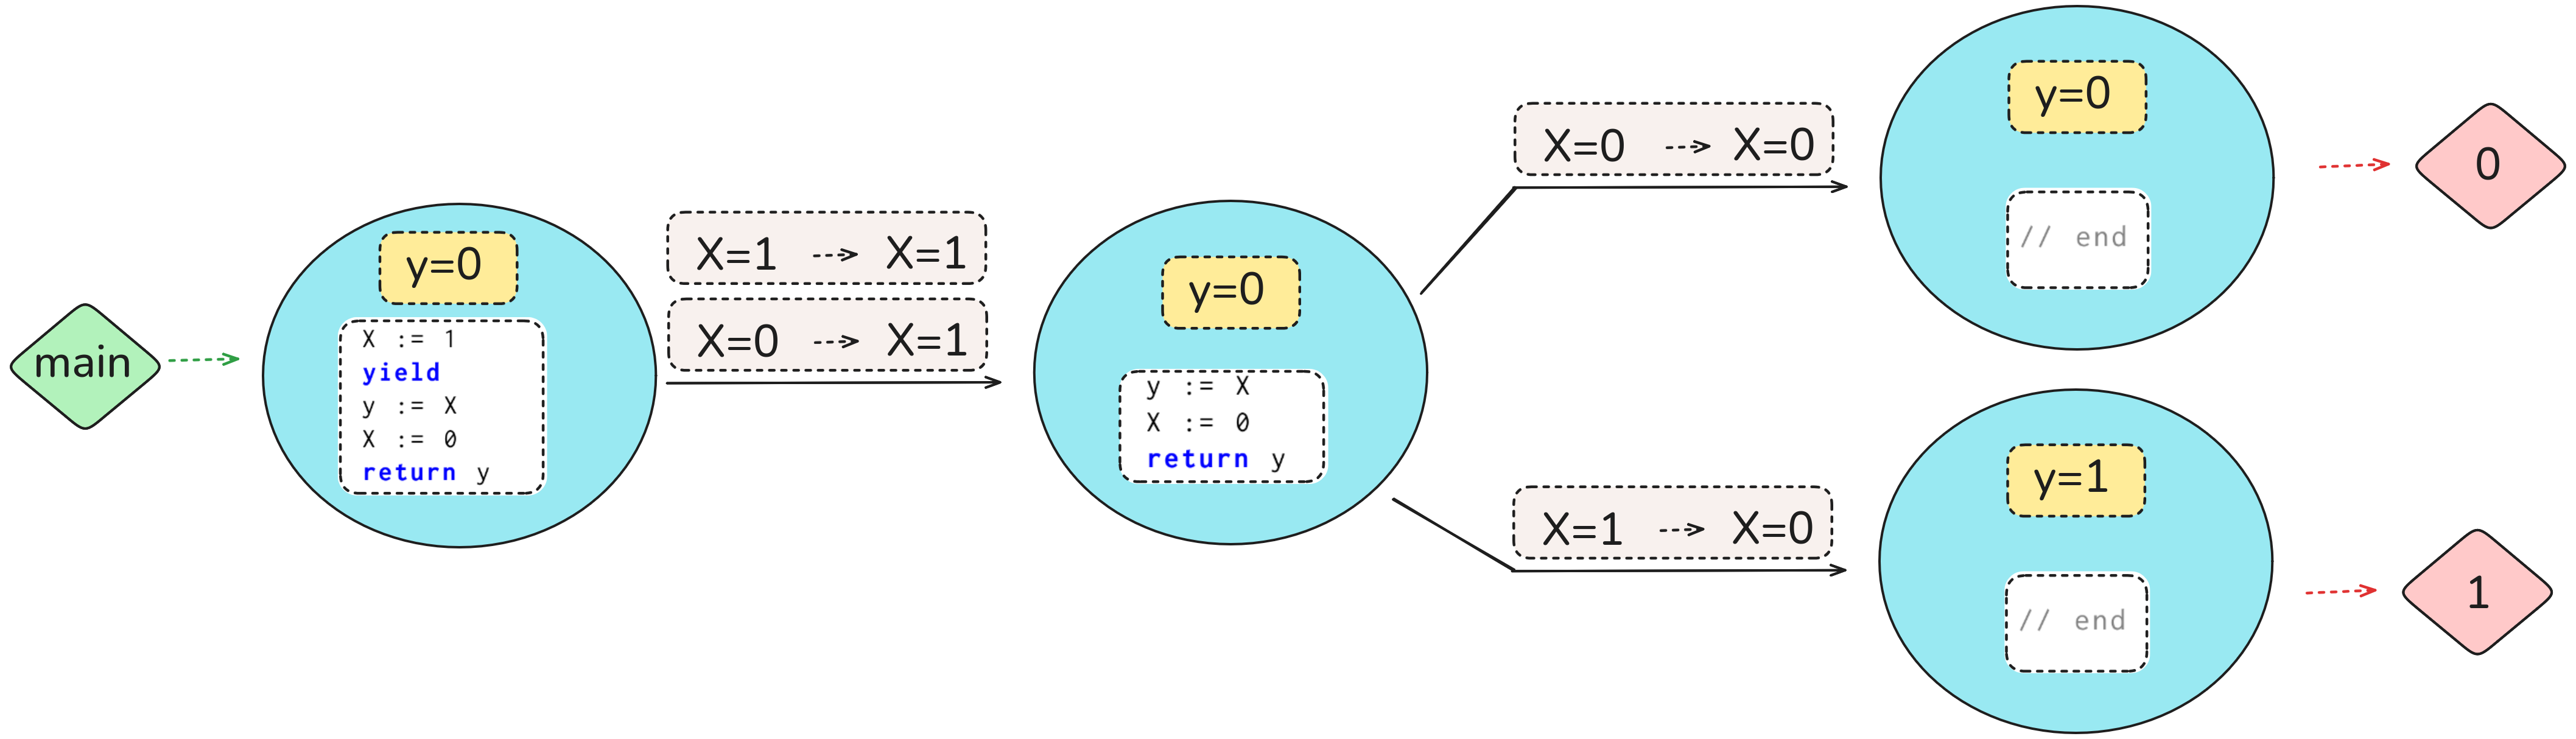
\includegraphics[width=1.1\textwidth]{plots/code_2_NS.png}
	\caption{Network System for the program in Listing~\ref{lst:MotivatingExample2NonSer}.}
	\label{fig:code2ExampleNS}
\end{figure}

%
%%
%The NS allows us to also extract the NFA encoding all serial executions. The states encode the global variable values, and the edges encode request/response pairs for all serial executions. As can be seen, serial executions can produce only pairs of the type ({\color{ForestGreen}$\blacklozenge_\text{main}$/{\color{red}$\blacklozenge_1$}}):
%
%\begin{figure}[!htbp]
%	\centering
%	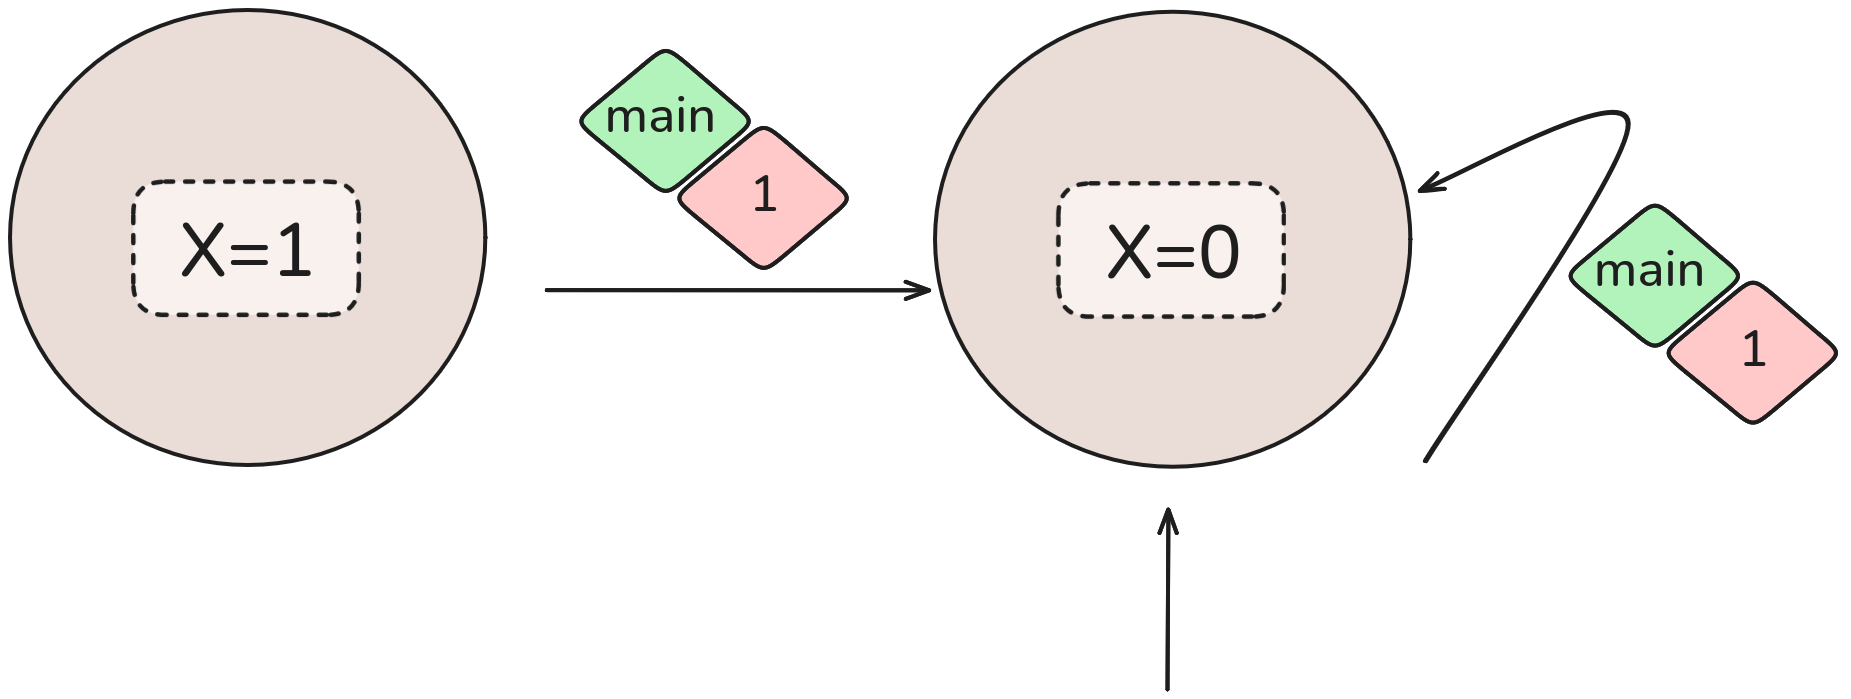
\includegraphics[width=0.5\textwidth,trim=0 0 0 0,clip]{plots/code_2_NFA.png}
%	\caption{NFA for serialized executions of Listing~\ref{lst:MotivatingExample2NonSer} program.}
%	\label{fig:code2ExampleNFA}
%\end{figure}
%
%Finally, the NS allows to generate the following Petri Net, encoding all possible interleavings of our program:
%
%\begin{figure}[!htbp]
%	\centering
%	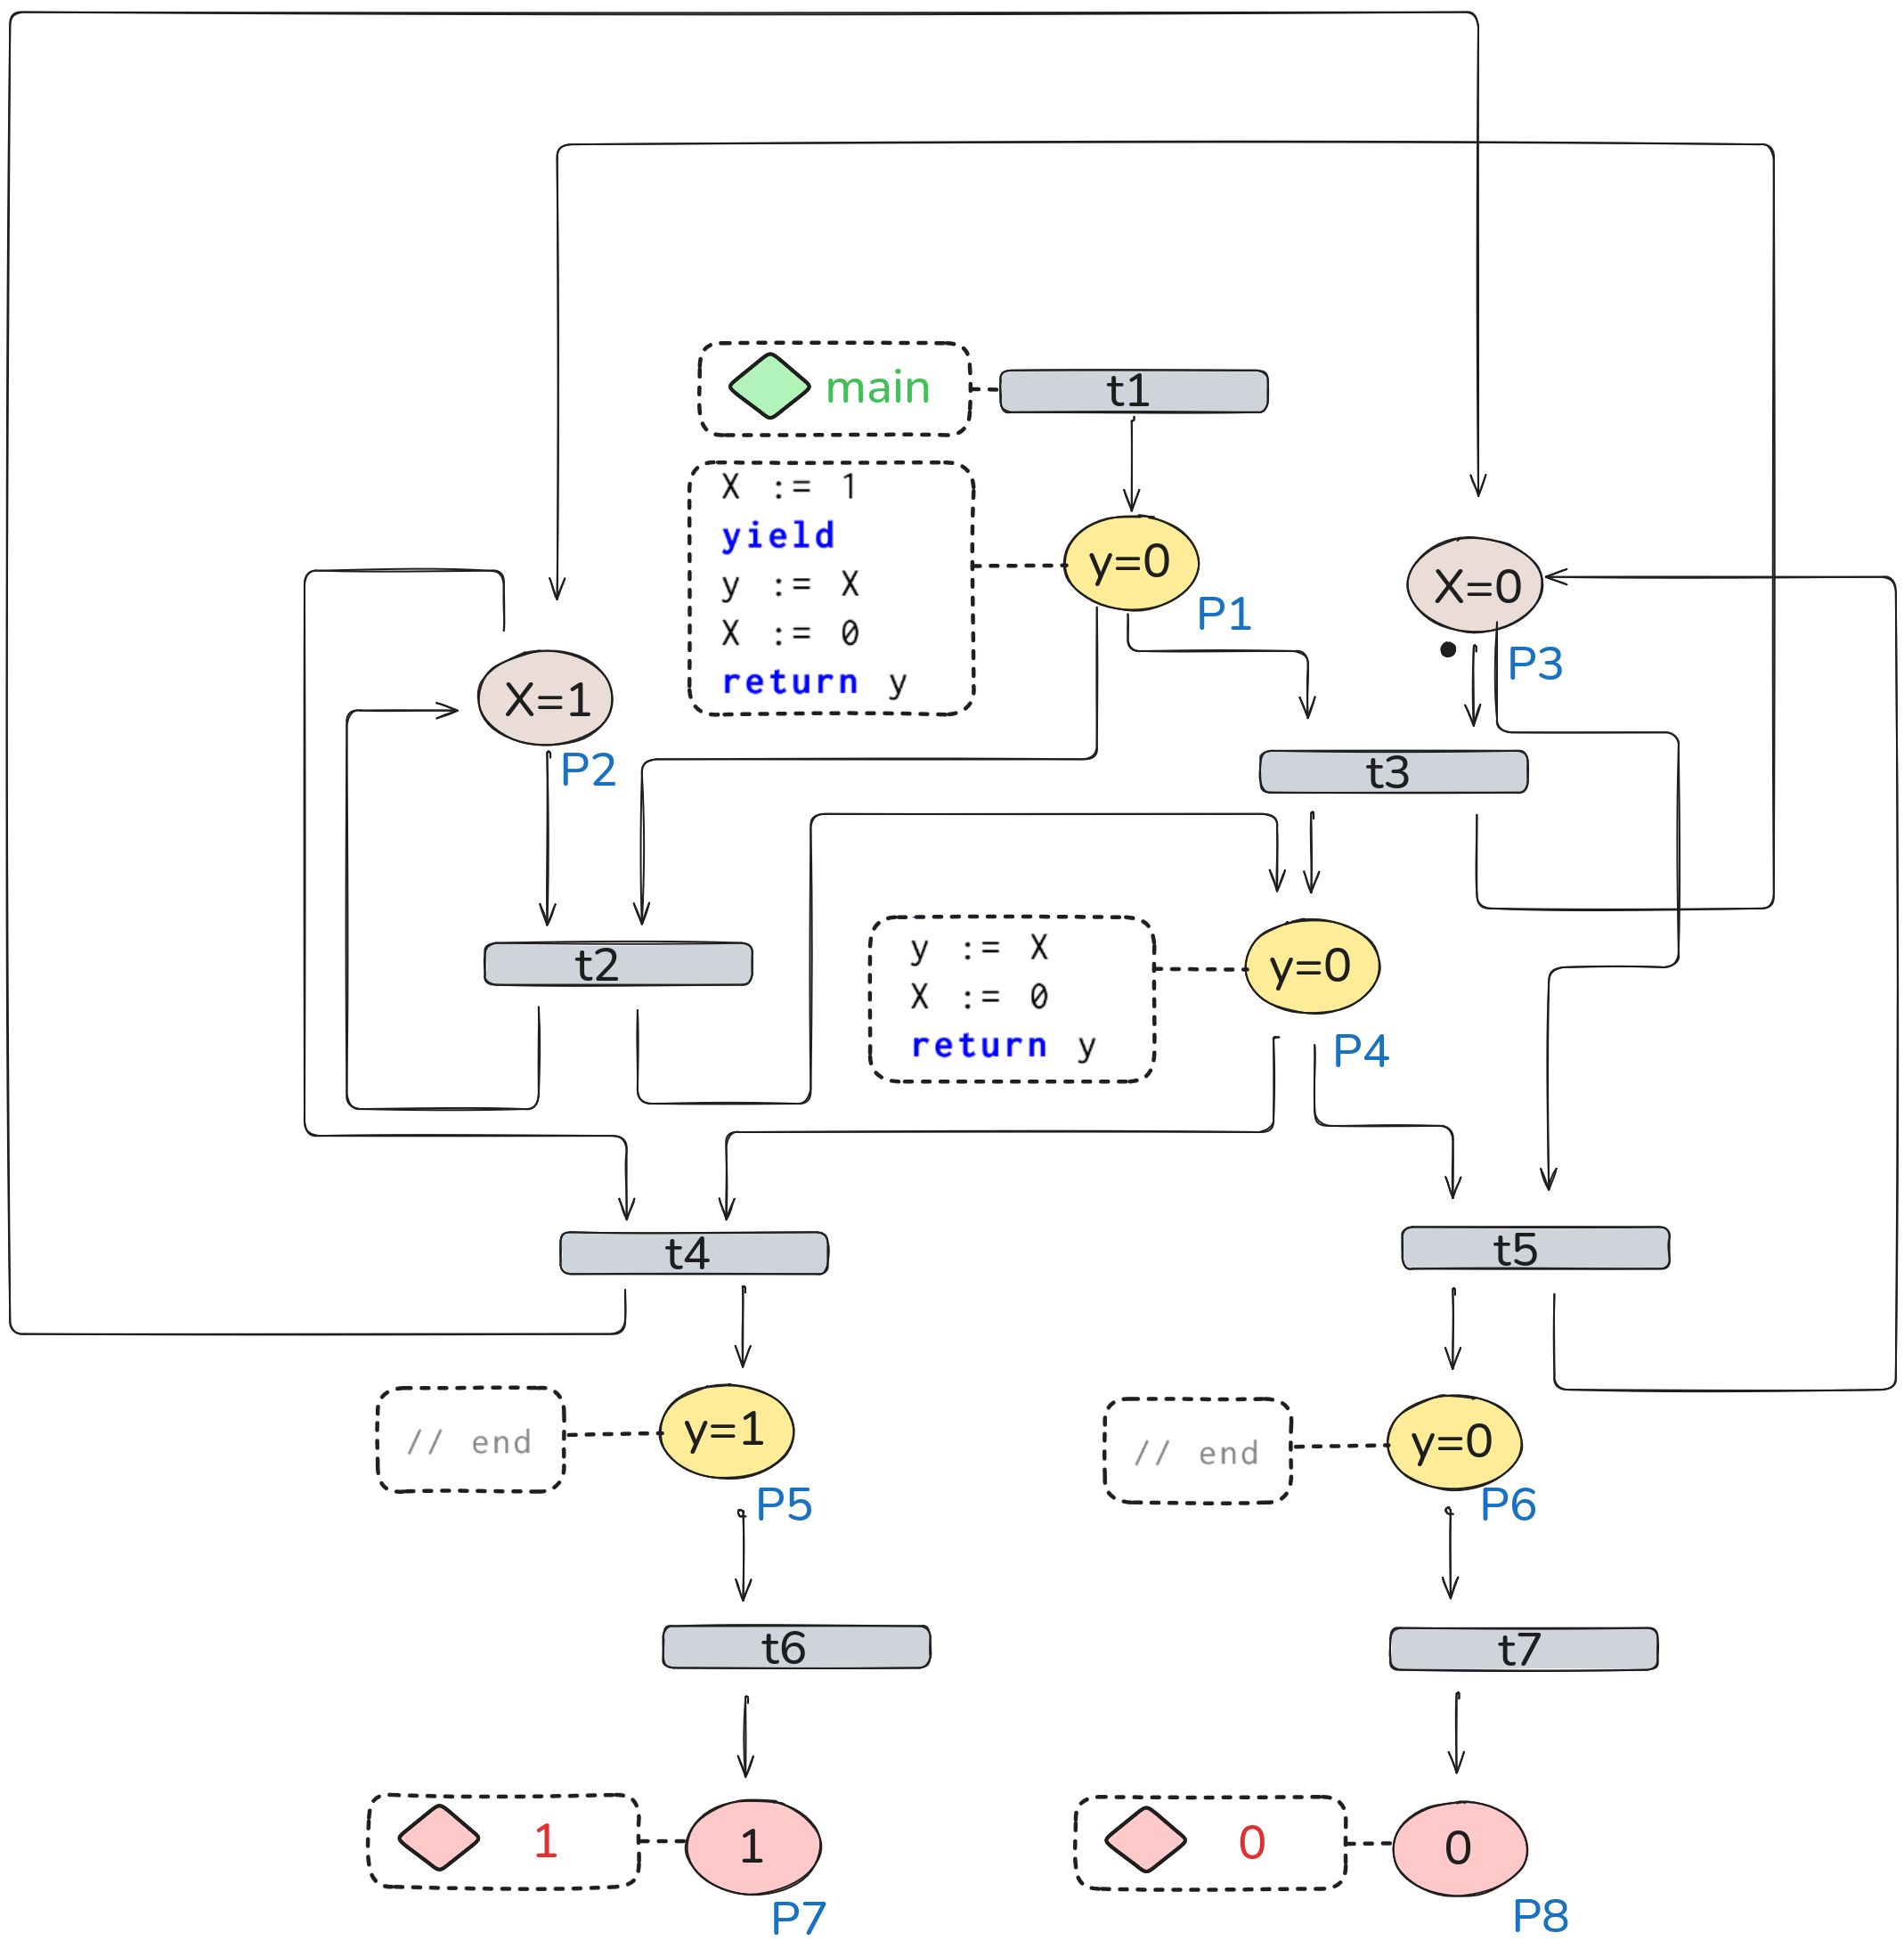
\includegraphics[width=0.7\textwidth]{plots/code_2_PN_with_annotation.png}
%	\caption{Petri Net for interleaving executions of Listing~\ref{lst:MotivatingExample2NonSer} program. Note that there is no firing sequence that can reach the place representing a response of ``0'', i.e., the bottom right place.}
%	\label{fig:code2ExamplePN}
%\end{figure}
%
%The places represent the $\delta$ transitions of our NS --- encoding either a ``step'' of our program, or spawning a request ($t_1$, which  corresponds to spawning request {\color{ForestGreen}$\blacklozenge_\text{main}$}), or returning a responds, e.g. transitions $t_6,t_7$ that corresponds to outputting responses {\color{red}$\blacklozenge_1$},{\color{red}$\blacklozenge_0$}.
%%
%Some places (\textcolor{blue}{$P_2$},\textcolor{blue}{$P_3$}) corresponds to the global state, while others ($P_1,P_4,P_5,P_6$) corresponds to the local state of an in-flight request.
%%
%Each token corresponds to a single packet, or (in the case of the global-variable-encoding places), to the global state of the program.
%
%
%
%Regarding the aforementioned program, we automatically generate the following LTL reachability query for the Petri net of Figure~\ref{fig:code1ExamplePN} (which, if satisfiable, indicates the program is not serializable):
%
%\todo{fix the "exists Marking M"}
%
%\[
%\exists\,M.\; 
%P_1 = 0 \wedge 
%\textcolor{blue}{P_2} \ge 0 \wedge \textcolor{blue}{P_3} \ge 0  \wedge P_4 = 0
%\wedge P_5 = 0 \wedge P_6 = 0 \wedge \textcolor{red}{P_7} = 0 \wedge \textcolor{red}{P_8} \ge 1.
%\]
%This asserts the existence of a marking with no tokens on $P_1,P_4,P_5,P_6$, exactly zero tokens on $\textcolor{red}{P_7}$, at least one token on $\textcolor{red}{P_8}$, and arbitrary tokens on $\textcolor{blue}{P_2},\textcolor{blue}{P_3}$.  In fact, the target marking
%\[
%M^* = \{\textcolor{blue}{P_3}(1),\;\textcolor{red}{P_7}(1),\;\textcolor{red}{P_8}(1)\}
%\]
%is reachable.  Table~\ref{tab:PetriNetFiringCounterexample} lists a firing sequence that leads to $M^*$.
%
%
%
%
%
%\begin{table}[H]
%	\centering
%	\label{tab:reach-seq}
%	\begin{tabular}{c l c c c c c c}
%		\toprule
%		\textbf{Step} 
%		& \textbf{Firing} 
%		& \multicolumn{3}{c}{\textbf{Marking (after firing)}} 
%		& \multicolumn{3}{c}{\textbf{Description (after firing)}} \\
%		\cmidrule(lr){3-5} \cmidrule(lr){6-8}
%		& 
%		& \textbf{Global} 
%		& \textbf{Local} 
%		& \textbf{Responses} 
%		& \textbf{Global state} 
%		& \textbf{In-flight packets} 
%		& \textbf{Responses} \\
%		\midrule
%		0 & --                                  
%		& {\color{blue}$P_3$(1)}                  
%		& --                                    
%		& --                                    
%		& {\color{blue}[X=0]}                   
%		& --                          
%		& --                                    \\
%		1 & $t_1$ 
%		& {\color{blue}$P_3$(1)}                  
%		& $P_1$(1)                                
%		& --                                    
%		& {\color{blue}[X=0]}                   
%		& {\color{ForestGreen}$\blacklozenge_\text{main}$} 
%		& --                                    \\
%		2 & $t_1$ 
%		& {\color{blue}$P_3$(1)}                  
%		& $P_1$(2)                                
%		& --                                    
%		& {\color{blue}[X=0]}                   
%		& {\color{ForestGreen}$\blacklozenge_\text{main}$}, {\color{ForestGreen}$\blacklozenge_\text{main}$}  
%		& --                                    \\
%		3 & $t_3$                                  
%		& {\color{blue}$P_2$(1)}                  
%		& $P_1$(1),$P_4$(1)                          
%		& --                                   
%		&                                    {\color{blue}[X=1]}    
%		&                                    {\color{black}$\blacklozenge_\text{until yield}$}, {\color{ForestGreen}$\blacklozenge_\text{main}$}   
%		& --                                    \\
%		4 & $t_2$                                  
%		& {\color{blue}$P_2$(1)}                  
%		& $P_4$(2)                                
%		& --                                    
%		&                                    {\color{blue}[X=1]}    
%		&                                    {\color{black}$\blacklozenge_\text{until yield}$}, {\color{black}$\blacklozenge_\text{until yield}$}   
%		& --                                    \\
%		5 & $t_4$                                  
%		& {\color{blue}$P_3$(1)}                  
%		& $P_5$(1),$P_4$(1)                          
%		& --                                    
%		&                                   {\color{blue}[X=0]}     
%		&                                    {\color{black}$\blacklozenge_\text{after yield}$}, {\color{black}$\blacklozenge_\text{until yield}$}   
%		& --                                    \\
%		6 & $t_6$                     
%		& {\color{blue}$P_3$(1)}                  
%		& $P_4$(1)                                
%		& {\color{red}$P_7$(1)}                    
%		&                                      	{\color{blue}[X=0]}  
%		&                                    {\color{black}$\blacklozenge_\text{until yield}$}   
%		&                                   {\color{red}$\blacklozenge_1$}     \\
%		7 & $t_5$                                  
%		& {\color{blue}$P_3$(1)}                  
%		& $P_6$(1)                                
%		& {\color{red}$P_7$(1)}                    
%		&                                   {\color{blue}[X=0]}    
%		&                                    {\color{black}$\blacklozenge_\text{after yield}$}      
%		&                                   {\color{red}$\blacklozenge_1$}        \\
%		8 & $t_7$                     
%		& {\color{blue}$P_3$(1)}                                  
%		& --                                    
%		& {\color{red}$P_7$(1),\color{red}$P_8$(1)}    
%		&                                   {\color{blue}[X=0]}    
%		&                                   --    
%		&                                   {\color{red}$\blacklozenge_0$}, {\color{red}$\blacklozenge_1$}       \\
%		\bottomrule
%	\end{tabular}
%		\caption{Firing sequence reaching the target marking $M^*$. The marking $P_i(n_j)$ indicates that there are $n_j$ tokens on place $P_i$. The initial marking has a single token in the place encoding the initialized values of the global variables.}
%		\label{tab:PetriNetFiringCounterexample}
%\end{table}
%
%%\newpage
%
%\subsection{NS Example: Serializability Proof}
%\label{sec:ns-serializable}
%
%Now, we observe again the adjusted program (as previously described in Listing~\ref{lst:MotivatingExample3Ser}):
%
%We present the corresponding Network System, Serailizability NFA, and Interleaving Petri Net in Appendix~\ref{appendix:MoreNsExamples}.
%
%Non-serializability corresponds to the above Petri Net being able to reach the following marking:
%
%\[
%\exists\,M.\; \textcolor{blue}
%P_1 = 0 \wedge 
%{P_2} \ge 0 \wedge \textcolor{blue}{P_3} \ge 0  \wedge P_4 = 0
%\wedge P_5 = 0 \wedge P_6 = 0 \wedge \textcolor{red}{P_7} = 0 \wedge \textcolor{red}{P_8} \ge 1.
%\]
%
%
%Note that this happened to be the exact same property as encoding non-serializability in the previous example, however, the Petri Net places $(P_1,\ldots,P_8)$ encode different states that correspond to the updated program. For example, now each place in the PN that encodes a global state accounts for two global variables, $X$ and $L$. 
%%
%However, this semilinear encoding (of non serializability) is \textit{unreachable}, as witness by the following inductive invariant:
%
%
%\[
%\begin{aligned}
%	&(P_{1},\textcolor{blue}{P_{2}},\textcolor{blue}{P_{3}},P_{4},P_{5},P_{6},\textcolor{red}{P_{7}},\textcolor{red}{P_{8}})
%	\;\mapsto\;\\
%	&\quad
%	\exists\,e_{0},\dots,e_{5}\ge0.\;
%	\Bigl(
%	e_{2}-e_{1}+\textcolor{blue}{P_{3}}-1=0\;\land\;
%	e_{2}+P_{1}-e_{5}=0\;\land\;
%	P_{5}-e_{1}+e_{4}=0\;\land\\
%	&\qquad\quad
%	-\,e_{4}+\textcolor{red}{P_{7}}=0\;\land\;
%	P_{6}+e_{3}-e_{0}=0\;\land\;
%	\textcolor{red}{P_{8}}-e_{3}=0\;\land\\
%	&\qquad\quad
%	-\,e_{2}+e_{1}+e_{0}+P_{4}=0\;\land\;
%	-\,e_{2}+e_{1}+\textcolor{blue}{P_{2}}=0
%	\Bigr)
%	\;\land\;
%	\bigl(P_{4}-1\ge0\;\lor\;\textcolor{blue}{P_{3}}-1\ge0\bigr).
%\end{aligned}
%\]
%
%
%We then revert this invariant to match our Network System, and project it to inputs/outputs of the system.
%%
%We get the following inductive invariants for each of the two global state:
%
%\begin{proof}
%	
%	\medskip\noindent
%	For global state \textcolor{blue}{[L=0,X=0]}
%	the projected invariant is:
%	\[
%	\bigl(\,\text{\color{ForestGreen}$\blacklozenge_{\text{main}}$}/\text{\color{red}$\blacklozenge_{0}$},\;
%	\text{\color{ForestGreen}$\blacklozenge_{\text{main}}$}/\text{\color{red}$\blacklozenge_{1}$}\bigr)
%	\;\mapsto\;
%	\exists\,e_{0},\dots,e_{5}\ge0.\;
%	\begin{aligned}[t]
%		& e_{2}-e_{1}=0,\quad
%		e_{2}-e_{5}=0,\quad
%		-e_{1}+e_{4}=0,\\
%		& -e_{4}+\bigl(\text{\color{ForestGreen}$\blacklozenge_{\text{main}}$}/\text{\color{red}$\blacklozenge_{1}$}\bigr)=0,\quad
%		-e_{0}+e_{3}=0,\quad
%		-e_{3}+\bigl(\text{\color{ForestGreen}$\blacklozenge_{\text{main}}$}/\text{\color{red}$\blacklozenge_{0}$}\bigr)=0,\\
%		& -e_{2}+e_{1}+e_{0}=0,\quad
%		-e_{2}+e_{1}=0.
%	\end{aligned}
%	\]
%	From these:
%	\[
%	e_{1}=e_{2}=e_{4}=e_{5}=(\;
%	\text{\color{ForestGreen}$\blacklozenge_{\text{main}}$}/\text{\color{red}$\blacklozenge_{1}$}),\;
%	e_{0}=e_{3}=
%	(\text{\color{ForestGreen}$\blacklozenge_{\text{main}}$}/\text{\color{red}$\blacklozenge_{0}$}),
%	\]
%	and
%	\[
%	-e_{2}+e_{1}+e_{0}=0\;\Longrightarrow\;e_{0}=0.
%	\]
%	Thus
%	\[
%(	\text{\color{ForestGreen}$\blacklozenge_{\text{main}}$}/\text{\color{red}$\blacklozenge_{0}$})
%	=0,
%	\]
%	so (\(\text{\color{ForestGreen}$\blacklozenge_{\text{main}}$}/\text{\color{red}$\blacklozenge_{0}$}\)) cannot be attained from the global state
%	\textcolor{blue}{[L=0,X=0]}.
%	
%	\medskip\noindent
%	Case 2: Global state \textcolor{blue}{[L=1,X=1]}.
%	The projected invariant is:
%	
%	
%	\[
%	\bigl(\,\text{\color{ForestGreen}$\blacklozenge_{\text{main}}$}/\text{\color{red}$\blacklozenge_{0}$},\;
%	\text{\color{ForestGreen}$\blacklozenge_{\text{main}}$}/\text{\color{red}$\blacklozenge_{1}$}\bigr)
%	\;\mapsto\;
%	\exists\,e_{0},\dots,e_{5}.\;\bot,
%	\]
%	which is unsatisfiable.  Hence, no completed‐request pair, and in particular no (\(\text{\color{ForestGreen}$\blacklozenge_{\text{main}}$}/\text{\color{red}$\blacklozenge_{0}$}\)) pair can occur in this state.
%	
%	\medskip\noindent
%	\textbf{Conclusion.}
%	In all reachable states
%	it holds that there cannot be any request/response pairs of type
%(	$	\text{\color{ForestGreen}$\blacklozenge_{\text{main}}$}/\text{\color{red}$\blacklozenge_{0}$}
%	$).
%	%
%	Furthermore, this indicates that the only attainable request/response pairs are of the form 	($	\text{\color{ForestGreen}$\blacklozenge_{\text{main}}$}/\text{\color{red}$\blacklozenge_{1}$})
%	$, which are in the language of of NFA for serial executions. Thus, this program is serializable.
%	%
%	We further show that these invariants are \textit{inductive}: they encompass the system’s initial state and, once satisfied, remain true for all subsequent executions.
%\end{proof}



%\newpage